\LaTeX{} is een softwaresysteem vergelijkbaar met een tekstverwerker zoals Microsoft Word. In de wetenschappelijke wereld is dit een zeer populaire software omdat het uitblinkt in het maken van technische documenten. \LaTeX{} is een markup\hyp{}taal.

Ik kwam als eerste in contact met \LaTeX{} door de standaard tekstverwerker van Mac, genaamd Pages. In deze tekstverwerker kan je wiskundige formules toevoegen in een \LaTeX{}\hyp{}notatie. Ik probeerde de code die ik online vond te ontleden en kon zo mijn eigen wiskundige formules schrijven in deze taal.

Later kwam ik er achter dat \LaTeX{} niet enkel een gebruikt kan worden voor wiskundige formules, maar dat het ook als volwaardige tekstverwerker kan functioneren. Omdat zeer veel papers geschreven worden met \LaTeX{}, besloot ik om mijn eindwerk ermee te schrijven. Dit zorgde dat ik meer onderzoek moest gaan doen naar hoe ik dit kon realiseren.

\LaTeX{} is het meest gebruikte macropakket van \TeX{}. \TeX{} is ontwikkeld in de jaren 70 door Donald Knuth om op een relatief eenvoudige manier het beschrijven van een ingewikkelde lay\hyp{}out mogelijk te maken. \TeX{} en dus ook \LaTeX{} zijn WYMIWYG, "What you mean is what you get", in tegenstelling tot andere WYSIWYG, "What you see is what you get", tekstverwerkers. Net zoals computerprogramma's moet een \TeX{}\hyp{}document gecompileerd worden om het resultaat te krijgen. De conventie is het compileren naar een pdf\hyp{}bestand.

De macro's in het \LaTeX{}\hyp{}pakket zijn voorgedefinieerde combinaties van commando's om het opmaakproces te versnellen. De schrijver kan deze macro's niet alleen gebruiken, maar zo ook aanpassen zijn zijn precieze nood. De mogelijkheid tot het schrijven van eigen macro's is natuurlijk ook een optie.

Het gehele idee achter het opmaken van een bestand in \LaTeX{} is dat je op voorhand bepaalde regels definieert en je gedurende het hele schrijfproces, je geen rekening meer moet houden met de opmaak. Zo krijg je een consistente lay\hyp{}out doorheen je bestand zonder al te veel moeite. Het versimpelt ook het wijzigen van de lay\hyp{}out omdat het op één globale plaats staat gedefinieerd.

Als oefening begon ik met het namaken van de gekregen templates voor documenten tijdens de stage in \LaTeX{}\hyp{}formaat. Deze documenten waren: het stageportfolio, de projectomschrijving en uiteindelijk het eindwerk zelf. Opdat ik meer met de taal werkte en meer onderzoek ernaar deed, kwam ik regelmatig op bevindingen die ervoor zorgde dat mijn hele structuur veranderde. Maar deze veranderingen zorgden er iedere keer voor dat het opmaakproces makkelijker en makkelijker werd.

\begin{figure}[!h]
  \centering
  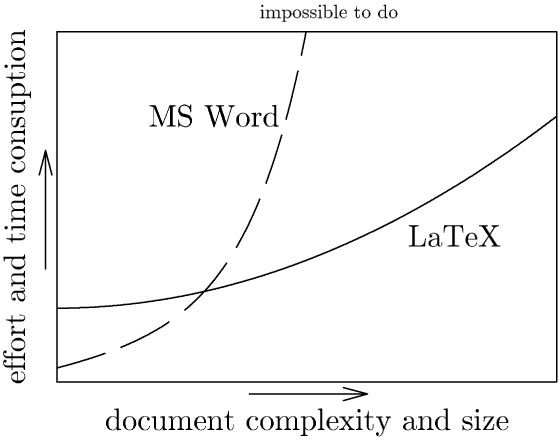
\includegraphics[width=0.48\linewidth]{images/latex/ms_word_vs_latex.png}
\end{figure}

\LaTeX{} heeft naar mijn mening een redelijk steile leercurve, maar eenmaal hier over kan je  er de vruchten van plukken. Voor de opmaak van mijn stageportfolio en mijn projectomschrijving heb ik wat meer tijd gestoken in vergelijking dat ik het met een tekstverwerker deed die ik reeds kende. Maar voor het eindwerk van de stage en het portfolio van iTalent heeft dit zeer veel tijd uitgespaard omdat ik praktisch geen rekening meer moest houden met het maken en volgen van de lay\hyp{}outregels.

Het idee achter het schrijven van mijn eindwerk in \LaTeX{} is dat ik na mijn bacheloropleiding wil doorschakelen naar een masteropleiding. Hier ga ik een master thesis voor moeten schrijven en om mij zo veel mogelijk te kunnen concentreren op het effectief schrijven en niet zo zeer op het opmaken van het document, zou ik deze in \LaTeX{} schrijven. Het lijkt mij ook een goed idee, want er worden veel master thesissen geschreven in \LaTeX{}. Dus het mijn eindwerk van mijn bacheloropleiding is de ideale voorbereiding voor mijn master thesis.

Nog een groot voordeel dat ik voordien niet wist is het gebruik van Bib\TeX{}. Dit is een soort van extensie op \LaTeX{} voor het aanleggen van literatuurlijsten. Google Scholar, een internetzoekmachine voor wetenschappelijke teksten en artikels, heeft een functie waarmee het gezochte bronnen kan citeren in een Bib\TeX{}\hyp{}formaat. Zo hoef je zelf niet alle informatie uit dit artikel of deze tekst te halen.

Het leren van \LaTeX{} is voor mij zeer nuttig geweest. Ik heb hierdoor een andere kijk gekregen op het maken en opstellen van tekstdocumenten. In het algemeen verlies ik veel minder tijd met het opmaken en het verfijnen van de opmaak. Ook het toepassen van mijn opmaak gebeurt nu automatisch. Hierdoor heb ik meer tijd om te spenderen aan het effectief schrijven van de tekst. Niet alleen het document maar ook de achterliggende structuur is voor mij nu overzichtelijker en makkelijk te lezen.

Doordat ik nieuwsgierig ben van karakter, vind ik het spannend om nieuwe technologi"en te onderzoeken en te leren. Niet alleen om mijn kennis te verruimen en te groeien als informaticus, maar ook omdat ik er vaak positieve zaken uit haal die ik initieel niet had verwacht. Mijn doel is om zo performant mogelijk te werken en dus zo weinig mogelijk tijd te verliezen met zaken die in mijn ogen niet nodig zijn. Met deze attitude zoek ik naar nieuwe technologi"en die mij verder kunnen helpen dit te bereiken. Ook mijn eigen uitdagen op zulke projecten geeft mij meer motivatie om er zo veel mogelijk uit te halen en is het voor mij geen moeite om er veel tijd in te steken.

Broncode iTalent portfolio: \url{https://github.com/VicSegers/iTalent-portfolio}